% This is samplepaper.tex, a sample chapter demonstrating the
% LLNCS macro package for Springer Computer Science proceedings;
% Version 2.20 of 2017/10/04
%
\documentclass[runningheads]{llncs}
%
%%%%%ДОБАВИЛ ДЛЯ РУССКОГО ТЕКСТА
\usepackage[utf8x]{inputenc}
\usepackage[english,russian]{babel}
\usepackage{cmap}
%%%%%
\usepackage{graphicx}

% Used for displaying a sample figure. If possible, figure files should
% be included in EPS format.
%
% If you use the hyperref package, please uncomment the following line
% to display URLs in blue roman font according to Springer's eBook style:
% \renewcommand\UrlFont{\color{blue}\rmfamily}

\begin{document}
%
\title{Comparison of dimensionality reduction schemes for parallel global optimization algorithms\thanks{Выполнено при поддержке РНФ -...}}
%
%\titlerunning{Abbreviated paper title}
% If the paper title is too long for the running head, you can set
% an abbreviated paper title here
%
\author{Konstantin Barkalov \and
Vladislav Sovrasov \and
Ilya Lebedev \and}
%
\authorrunning{F. Author et al.}
% First names are abbreviated in the running head.
% If there are more than two authors, 'et al.' is used.
%
\institute{
Lobachevsky State University of Nizhny Novgorod, Nizhny Novgorod, Russia
\email{konstantin.barkalov@itmm.unn.ru}\\
\email{sovrasov.vlad@gmail.com}\\
\email{ilya.lebedev@itmm.unn.ru}\\
\url{http://hpc-education.unn.ru/основные-напраления/глобальная-оптимизация} }
%
\maketitle              % typeset the header of the contribution
%
\begin{abstract}
This work considers a parallel algorithms for solving multi-extremal optimization problems. Algorithms are developed within the framework of the information-statistical approach and implemented in a parallel solver “Globalizer” . The optimization problem is solved by reducing the multidimensional problem to a set of joint one-dimensional problems that are solved in parallel. Five types of Peano-type space-filling curves are employed to reduce dimension. The results of computational experiments carried out on several hundred test problems are discussed. 

\keywords{Global optimization \and  Dimension reduction \and Parallel algorithms  \and Multidimensional multiextremal optimization  \and Global search algorithms  \and Parallel computations }
\end{abstract}
%
%
%

\section{Introduction}\label{sec:intro}

Global (or multiextremal) optimization problems are among the most complex problems
in both theory and practice of optimal decision making. In these kinds of problems,
the optimization criterion can have several local optima within the search domain.
The existence of several local optima makes
finding the global optimum difficult essentially, since it requires examining the whole feasible
search domain. The volume of computations for solving global optimization problems
can increase exponentially with increasing number of varied parameters.
\par
These global optimization problem features impose special requirements on the quality
of the optimization methods and on the software to implement these ones. The global
optimization methods should be highly efficient, and the software systems should be developed on
a good professional basis. In general, the global optimization problems can be solved at
a reasonable time by employing parallel computations on modern supercomputing systems only.
\par
The general state of the art in the field of global optimization is presented in a
number of key monographs  \cite{floudasPardGO}, \cite{horstTuyGO}, \cite{locatelliSchoenGO}, \cite{pinterGO}, \cite{strSergGO}, \cite{zilinskTornGO}, \cite{zhigljavskyRandGO}.
The development of optimization methods, which use the high-performance computational
systems to solve the time-consuming global optimization problems, is an area of
intensive research --- see, for instance, \cite{censorZeniosParGO}, \cite{ciegisHentyParGO},
\cite{luqueAlbaGA}, \cite{stronginGergelBarkalovParGO}, \cite{strSergGO}. The obtained
theoretical results provide the efficient solutions of many applied global
optimization problems in various fields of scientific and technical applications \cite{Famularo1999}, \cite{fasanoPinter2013},
\cite{floudasPardalosGOState}, \cite{Kvasov2015}, \cite{Menniti}, \cite{locatelliSchoenGO},
\cite{luqueAlbaGA}, \cite{pardalosZhigljavskyZilinskas2016}, \cite{pinterGO}.
\par
At the same time, the practical implementation of these global optimization algorithms
within the framework of industrial software systems is quite limited. In many cases,
software implementations are experimental in nature and are used by the developers
themselves to obtain the results from the computational experiments required for the
scientific publications. This situation originates from high development costs of the
professional software systems, which can be used by numerous users. In addition, the global
optimization problems could be solved in an automatic mode rarely because of the
complexity of these ones. The user should actively control the global search
process that implies an adequate level of qualification in the field of optimization
(particularly, the user should know and understand the global optimization methods well).
\par
In this work, the authors consider an approach to minimizing multiextremal functions  developed in ...????????
This allows problems to be solved in which function values may not be deter-mined for the entire search domain. Under this approach, solving multidimen-sional problems is reduced (using Peano-type space-filling curves) to solving equivalent one-dimensional problems.
It should be noted that standard approaches to algorithm parallelization are not quite applicable to global optimization. For example, the rules for selecting an-other iteration point are quite simple and do not require parallelization (as over-heads associated with organizing parallel computations will nullify any possible acceleration). Some acceleration can be achieved by parallelizing the computa-tion of function values describing the object to be optimized; however, this ap-proach is specific to each individual problem being solved.
The following approach looks more promising. The algorithm can be modified to run several trials in parallel. This approach provides the efficiency (as paral-lelization is applied to the most computation-intensive part of the problem solv-ing process) and generality (in that it applies to a wide range of global optimiza-tion algorithms). The approach, described in  \cite{Two_Level_Parallel} for unconstrained optimization, was used in this work for parallelizing constrained optimization algorithms.

\section{Statement of Multidimensional Global Optimization Problem}

\section{Methods of Dimension Reduction}

\subsection{Базовый алгоритм}
s
\subsection{Сдвиговые}
s
\subsection{Вращаемые}
s
\subsection{Еще одни развертки}
s
\subsection{Гладкие}
s
\section{Parallel Computations for Solving Global Optimization Problems.}
\subsection{Core Multidimensional Algorithm of Global Search}
s
\subsection{Параллельные множественные отображения}
s
\section{Results of Numerical Experiments}
s
\subsection{Сравнение последовательных сдвиговых и вращаемых разверток}
s
\subsection{Параллельные вращаемые развертки}
s
\subsection{Параллельные вращаемые развертки для задач большой размерности}
s
\section{Вывод о целесообразности применения того или иного вида разверток для того или иного вида задач}
s

\section{First Section}
\subsection{A Subsection Sample}
Please note that the first paragraph of a section or subsection is
not indented. The first paragraph that follows a table, figure,
equation etc. does not need an indent, either.

Subsequent paragraphs, however, are indented.

\subsubsection{Sample Heading (Third Level)} Only two levels of
headings should be numbered. Lower level headings remain unnumbered;
they are formatted as run-in headings.

\paragraph{Sample Heading (Fourth Level)}
The contribution should contain no more than four levels of
headings. Table~\ref{tab1} gives a summary of all heading levels.

\begin{table}
\caption{Table captions should be placed above the
tables.}\label{tab1}
\begin{tabular}{|l|l|l|}
\hline
Heading level &  Example & Font size and style\\
\hline
Title (centered) &  {\Large\bfseries Lecture Notes} & 14 point, bold\\
1st-level heading &  {\large\bfseries 1 Introduction} & 12 point, bold\\
2nd-level heading & {\bfseries 2.1 Printing Area} & 10 point, bold\\
3rd-level heading & {\bfseries Run-in Heading in Bold.} Text follows & 10 point, bold\\
4th-level heading & {\itshape Lowest Level Heading.} Text follows & 10 point, italic\\
\hline
\end{tabular}
\end{table}


\noindent Displayed equations are centered and set on a separate
line.
\begin{equation}
x + y = z
\end{equation}
Please try to avoid rasterized images for line-art diagrams and
schemas. Whenever possible, use vector graphics instead (see
Fig.~\ref{fig1}).

\begin{figure}
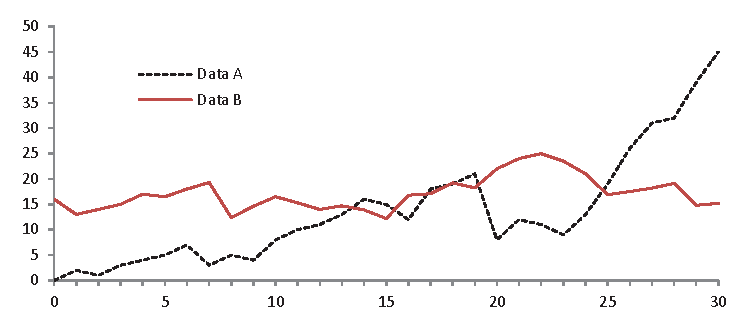
\includegraphics[width=\textwidth]{fig1.eps}
\caption{A figure caption is always placed below the illustration.
Please note that short captions are centered, while long ones are
justified by the macro package automatically.} \label{fig1}
\end{figure}

\begin{theorem}
This is a sample theorem. The run-in heading is set in bold, while
the following text appears in italics. Definitions, lemmas,
propositions, and corollaries are styled the same way.
\end{theorem}
%
% the environments 'definition', 'lemma', 'proposition', 'corollary',
% 'remark', and 'example' are defined in the LLNCS documentclass as well.
%
\begin{proof}
Proofs, examples, and remarks have the initial word in italics,
while the following text appears in normal font.
\end{proof}
For citations of references, we prefer the use of square brackets
and consecutive numbers. Citations using labels or the author/year
convention are also acceptable. The following bibliography provides
a sample reference list with entries for journal
articles~\cite{ref_article1}, an LNCS chapter~\cite{ref_lncs1}, a
book~\cite{ref_book1}, proceedings without editors~\cite{ref_proc1},
and a homepage~\cite{ref_url1}. Multiple citations are grouped
\cite{ref_article1,ref_lncs1,ref_book1},
\cite{ref_article1,ref_book1,ref_proc1,ref_url1}.
%
% ---- Bibliography ----
%
% BibTeX users should specify bibliography style 'splncs04'.
% References will then be sorted and formatted in the correct style.
%
% \bibliographystyle{splncs04}
% \bibliography{mybibliography}
%
\begin{thebibliography}{107}


\bibitem{barkalovGergel2014}
\newblock K. Barkalov and V. Gergel,
\newblock \emph{\emph{Multilevel scheme of dimensionality reduction for parallel global search algorithms}},
\newblock in \emph{Proceedings of the 1st International Conference on Engineering and Applied Sciences Optimization}, (2014), 2111--2124.

\bibitem{barkalovGergel2015}% (MR3539505) [10.1007/s10898-016-0411-y]
\newblock K. Barkalov and V. Gergel,
\newblock \emph{\emph{Parallel global optimization on GPU}},
\newblock \emph{J. Glob. Optim.}, \textbf{66} (2016), 3--20.

\bibitem{barkalovGergelLebedev2015} %[10.1007/978-3-319-21909-7_31]
\newblock K. Barkalov, V. Gergel and I. Lebedev,
\newblock \emph{\emph{Use of Xeon Phi coprocessor for solving global optimization problems}},
\newblock \emph{LNCS}, \textbf{9251} (2015), 307--318.

\bibitem{barkalovGergelLebedevSysoev2015}
\newblock K. Barkalov, V. Gergel, I. Lebedev and A. Sysoev,
\newblock \emph{\emph{Solving the global optimization problems on heterogeneous cluster systems}},
\newblock in \emph{CEUR Workshop Proceedings}, \textbf{1482} (2015), 411--419.

\bibitem{Barkalov2013}% [10.1007/978-3-642-39958-9_14]
\newblock K. Barkalov, A. Polovinkin, I. Meyerov, S. Sidorov and N. Zolotykh,
\newblock \emph{\emph{SVM regression parameters optimization using parallel global search algorithm}},
\newblock \emph{LNCS}, \textbf{7979} (2013), 154--166.

\bibitem{bussieckMeeraus2004} (MR3618583)% [10.1007/978-1-4613-0215-5_8]
\newblock M. R. Bussieck and A. Meeraus,
\newblock \emph{\emph{General algebraic modeling system (GAMS)}},
\newblock in \emph{Modeling Languages in Mathematical Optimization} (ed. J. Kallrath), Springer, (2004), 137--157.

\bibitem{censorZeniosParGO}% (MR1486040)
\newblock Y. Censor and S. A. Zenios,
\newblock \emph{Parallel Optimization: Theory, Algorithms, and Applications},
\newblock Oxford University Press, 1998.

\bibitem{ciegisHentyParGO} (MR2499546)% [10.1007/978-0-387-09707-7]
\newblock R. \v Ciegis, D. Henty, B. K\aa gstr\"om and J. \v Zilinskas,
\newblock \emph{Parallel Scientific Computing and Optimization: Advances and Applications},
\newblock Springer, 2009.

\bibitem{iosoDescription}
\newblock I. N. Egorov, G. V. Kretinin, I. A. Leshchenko and S. V. Kuptzov,
\newblock \emph{\emph{IOSO optimization toolkit --- novel software to create better design}},
\newblock in \emph{9th AIAA/ISSMO Symposium on Multidisciplinary Analysis and Optimization}, 2002. Available from \url{http://www.iosotech.com/text/2002\_4329.pdf}.

\bibitem{Famularo1999} %(MR1827451) [10.1016/S0005-1098(99)00058-8]
\newblock D. Famularo, P. Pugliese and Y. D. Sergeyev,
\newblock \emph{\emph{A global optimization technique for checking parametric robustness}},
\newblock \emph{Automatica}, \textbf{35} (1999), 1605--1611.

\bibitem{fasanoPinter2013}% (MR3013800) [10.1007/978-1-4614-4469-5]
\newblock G. Fasano and J. D. Pint\'er,
\newblock \emph{Modeling and Optimization in Space Engineering},
\newblock Springer, 2013.

\bibitem{floudasPardalosGOState} %(MR1390521) [10.1007/978-1-4613-3437-8]
\newblock C. A. Floudas and M. P. Pardalos,
\newblock \emph{State of the Art in Global Optimization: Computational Methods and Applications},
\newblock Kluwer Academic Publishers, Dordrecht, 1996.

\bibitem{floudasPardGO}% (MR1147432) [10.1007/s10898-008-9332-8]
\newblock C. A. Floudas and M. P. Pardalos,
\newblock \emph{Recent Advances in Global Optimization},
\newblock Princeton University Press, 2016.

\bibitem{Gablonsky} %(MR1856800) [10.1023/A:1017930332101]
\newblock J. M. Gablonsky and C. T. Kelley,
\newblock \emph{\emph{A locally-biased form of the DIRECT algorithm}},
\newblock \emph{J. Glob. Optim.}, \textbf{21} (2001), 27--37.

\bibitem{gavianoKvasovLeraSergeev2003} %(MR2077342) [10.1145/962437.962444]
\newblock M. Gaviano, D. E. Kvasov, D. Lera and Y. D. Sergeev,
\newblock \emph{\emph{Software for generation of classes of test functions with known local and global minima for global optimization}},
\newblock \emph{ACM Trans. Math. Software}, \textbf{29} (2003), 469--480.

\bibitem{gergelLebedev2015}% [10.1016/j.procs.2015.11.008]
\newblock V. Gergel and I. Lebedev,
\newblock \emph{\emph{Heterogeneous parallel computations for solving global optimization problems}},
\newblock \emph{Procedia Comput. Sci.}, \textbf{66} (2015), 53--62.

\bibitem{gergel1993}
\newblock V. Gergel,
\newblock \emph{\emph{A software system for multi-extremal optimization}},
\newblock \emph{Eur. J. Oper. Res.}, \textbf{65} (1993), 305--313.

\bibitem{gergel1996}% (MR1399766)
\newblock V. Gergel,
\newblock \emph{\emph{A method for using derivatives in the minimization of multiextremum functions}},
\newblock \emph{Comput. Math. Math. Phys.}, \textbf{36} (1996), 729--742.

\bibitem{gergel1997} %(MR1443089) [10.1023/A:1008290629896]
\newblock V. Gergel,
\newblock \emph{\emph{A global optimization algorithm for multivariate functions with Lipschitzian first derivatives}},
\newblock \emph{J. Glob. Optim.}, \textbf{10} (1997), 257--281.

\bibitem{gergel2013} %[doi:10.1016/j.procs.2013.05.164]
\newblock V. Gergel, et al.,
\newblock \emph{\emph{High performance computing in biomedical applications}},
\newblock \emph{Procedia Computer Science}, \textbf{18} (2013), 10--19.

\bibitem{gergel2015}% [10.15866/ireaco.v8i1.4935]
\newblock V. Gergel, et al.,
\newblock \emph{\emph{Recognition of surface defects of cold-rolling sheets based on method of localities}},
\newblock \emph{International Review of Automatic Control, } \textbf{8} (2015), 51--55.

\bibitem{gergelSidorov2015}% [10.1007/978-3-319-21909-7_49]
\newblock V. Gergel and S. Sidorov,
\newblock \emph{\emph{A two-level parallel global search algorithm for solving computationally intensive multi-extremal optimization problems}},
\newblock \emph{LNCS}, \textbf{9251} (2015), 505--515.

\bibitem{grishaginStrongin1984}% (MR785497)
\newblock V. A. Grishagin and R. G. Strongin,
\newblock \emph{\emph{Optimization of multi-extremal functions subject to monotonically unimodal constraints}},
\newblock \emph{Engineering Cybernetics}, \textbf{5} (1984), 117--122.

\bibitem{holmstromEdvall2004}% [10.1007/978-1-4613-0215-5_19]
\newblock K. Holmstrm and M. M. Edvall,
\newblock \emph{\emph{The TOMLAB optimization environment}},
\newblock \emph{Modeling Languages in Mathematical Optimization}, Springer, (2004), 369--376.

\bibitem{horstTuyGO}% (MR1102239) [10.1007/978-3-662-03199-5]
\newblock R. Horst and H. Tuy,
\newblock \emph{Global Optimization: Deterministic Approaches},
\newblock Springer-Verlag, Berlin, 1990.

\bibitem{Jones} (MR1246501)% [10.1007/BF00941892]
\newblock D. R. Jones, C. D. Perttunen and B. E. Stuckman,
\newblock \emph{\emph{Lipschitzian optimization without the Lipschitz constant}},
\newblock \emph{J. Optim. Theory Appl.}, \textbf{79} (1993), 157--181.

\bibitem{kearfott2009}%(MR2554906) [10.1080/10556780802614051]
\newblock R. B. Kearfott,
\newblock \emph{\emph{GlobSol user guide}},
\newblock \emph{Optim. Methods Softw.}, \textbf{24} (2009), 687--708.

\bibitem{Kvasov2015}% (MR3585540) [10.1016/j.advengsoft.2014.09.014]
\newblock D. E. Kvasov and Y. D. Sergeyev,
\newblock \emph{\emph{Deterministic approaches for solving practical black-box global optimization problems}},
\newblock \emph{Adv. Eng. Softw.}, \textbf{80} (2015), 58--66.

\bibitem{Menniti}% [10.1016/j.epsr.2007.10.009]
\newblock D. E. Kvasov, D. Menniti, A. Pinnarelli, Y. D. Sergeyev and N. Sorrentino,
\newblock \emph{\emph{Tuning fuzzy power-system stabilizers in multi-machine systems by global optimization algorithms based on
 efficient domain partitions}},
\newblock \emph{Electric Power Systems Research}, \textbf{78} (2008), 1217--1229.

\bibitem{Pizzuti}% (MR1971214) [10.1007/s00211-002-0419-8]
\newblock D. E. Kvasov, C. Pizzuti and Y. D. Sergeyev,
\newblock \emph{\emph{Local tuning and partition strategies for diagonal GO methods}},
\newblock \emph{Numerische Mathematik}, \textbf{94} (2003), 93--106.

\bibitem{liberti2009}% (MR2206955) [10.1007/0-387-30528-9_8]
\newblock L. Liberti,
\newblock \emph{\emph{Writing global optimization software}},
\newblock in \emph{Nonconvex Optimization and Its Applications}, Springer, \textbf{84} (2006), 211--262.


\bibitem{linSchrage2009}% (MR2554904) [10.1080/10556780902753221]
\newblock Y. Lin and L. Schrage,
\newblock \emph{\emph{The global solver in the LINDO API}},
\newblock \emph{Optim. Methods Softw.}, \textbf{24} (2009), 657--668.

\bibitem{locatelliSchoenGO}% (MR3136805) [10.1137/1.9781611972672]
\newblock M. Locatelli and F. Schoen,
\newblock \emph{Global Optimization: Theory, Algorithms and Applications},
\newblock SIAM, 2013.

\bibitem{luqueAlbaGA}% (MR2808873) [10.1007/978-3-642-22084-5]
\newblock G. Luque and E. Alba,
\newblock \emph{Parallel Genetic Algorithms. Theory and Real World Applications},
\newblock Springer-Verlag, Berlin, 2011.

\bibitem{mongeauKarsentyRouze2000} %(MR1785196) [10.1080/10556780008805783]
\newblock M. Mongeau, H. Karsenty, V. Rouz$\acute{e}$ and J. B. Hiriart-Urruty,
\newblock \emph{\emph{Comparison of public-domain software for black box global optimization}},
\newblock \emph{Optim. Methods Softw.}, \textbf{13} (2000), 203--226.

\bibitem{mullen2014} %[10.18637/jss.v060.i06]
\newblock K. M. Mullen,
\newblock \emph{\emph{Continuous global optimization in R}},
\newblock \emph{J. Stat. Softw.}, \textbf{60} (2014).

\bibitem{pardalosZhigljavskyZilinskas2016}% (MR2361744) [10.1007/978-3-319-29975-4]
\newblock M. P. Pardalos, A. A. Zhigljavsky and J. \v Zilinskas,
\newblock \emph{Advances in Stochastic and Deterministic Global Optimization},
\newblock Springer, 2016.

\bibitem{pinterGO}% (MR1374104) [10.1007/978-1-4757-2502-5]
\newblock J. D. Pint\'er,
\newblock \emph{Global Optimization in Action (Continuous and Lipschitz Optimization: Algorithms, Implementations and Applications)},
\newblock Kluwer Academic Publishers, Dordrecht, 1996.

\bibitem{pinter2009}% (MR2528693)
\newblock J. D. Pint\'er,
\newblock \emph{\emph{Software development for global optimization}},
\newblock \emph{Lectures on Global Optimization. Fields Institute Communications}, \textbf{55} (2009), 183--204.

\bibitem{riosSahinidis2013} %(MR3070154) [10.1007/s10898-012-9951-y]
\newblock L. M. Rios and N. V. Sahinidis,
\newblock \emph{\emph{Derivative-free optimization: a review of algorithms and comparison of software implementations}},
\newblock \emph{J. Glob. Optim.}, \textbf{56} (2013), 1247--1293.

\bibitem{sahinidis1996} %(MR1376505) [10.1007/BF00138693]
\newblock N. V. Sahinidis,
\newblock \emph{\emph{BARON: A general purpose global optimization software package}},
\newblock \emph{J. Glob. Optim.}, \textbf{8} (1996), 201--205.

\bibitem{sergeyev1995} %(MR1358808) [10.1137/0805041]
\newblock Y. D. Sergeyev,
\newblock \emph{\emph{An information global optimization algorithm with local tuning}},
\newblock \emph{SIAM J. Optim.}, \textbf{5} (1995), 858--870.

\bibitem{sergeyev1999}% (MR1699326)
\newblock Y. D. Sergeyev,
\newblock \emph{\emph{Multidimensional global optimization using the first derivatives}},
\newblock \emph{Comput. Math. Math. Phys.}, \textbf{39} (1999), 743--752.

\bibitem{sergeyevKvasov2006}% (MR2197562) [10.1137/040621132]
\newblock Y. D. Sergeyev and D. E. Kvasov,
\newblock \emph{\emph{Global search based on efficient diagonal partitions and a set of Lipschitz constants}},
\newblock \emph{SIAM Journal on Optimization}, \textbf{16} (2006), 910--937.

\bibitem{sergeyevGrishagin2001}% (MR1825071) [10.1023/A:1010185125012]
\newblock Y. D. Sergeyev and V. A. Grishagin,
\newblock \emph{\emph{Parallel asynchronous global search and the nested optimization scheme}},
\newblock \emph{J. Comput. Anal. Appl.}, \textbf{3} (2001), 123--145.

\bibitem{sergeyevStronginLera2013}% (MR3113120) [10.1007/978-1-4614-8042-6]
\newblock Y. D. Sergeyev, R. G. Strongin and D. Lera,
\newblock \emph{Introduction to Global Optimization Exploiting Space-filling Curves},
\newblock Springer, 2013.

\bibitem{Famularo2001}% (MR1866703) [10.1023/A:1012391611462]
\newblock Y. D. Sergeyev, D. Famularo and P. Pugliese,
\newblock \emph{\emph{Index branch-and-bound algorithm for Lipschitz univariate global optimization with multiextremal constraints}},
\newblock \emph{J. Glob. Optim.}, \textbf{21} (2001), 317--341.

\bibitem{strongin1978}% (MR509033)
\newblock R. G. Strongin,
\newblock \emph{Numerical Methods in Multi-Extremal Problems (Information-Statistical Algorithms)},
\newblock Moscow: Nauka, In Russian, 1978.

\bibitem{strongin1992}% (MR1263606) [10.1007/BF00122428]
\newblock R. G. Strongin,
\newblock \emph{\emph{Algorithms for multi-extremal mathematical programming problems employing a set of joint space-filling curves}},
\newblock \emph{J. Glob. Optim.}, \textbf{2} (1992), 357--378.

\bibitem{stronginGergelBarkalovParGO}
\newblock R. G. Strongin, V. P. Gergel, V. A. Grishagin and K. A. Barkalov,
\newblock \emph{Parallel Computations for Global Optimization Problems},
\newblock Moscow State University (In Russian), Moscow, 2013.

\bibitem{strSergGO}5 (MR1797058) [10.1007/978-1-4615-4677-1]
\newblock R. G. Strongin and Y. D. Sergeyev,
\newblock \emph{Global Optimization with Non-convex Constraints. Sequential and Parallel Algorithms},
\newblock Kluwer Academic Publishers, Dordrecht (2000, 2nd ed. 2013, 3rd ed. 2014).

\bibitem{zilinskTornGO}% (MR1100586) [10.1007/3-540-50871-6]
\newblock A. T\"orn and A. \v Zilinskas,
\newblock \emph{Global Optimization},
\newblock Springer, 1989.

\bibitem{venkataraman2009}
\newblock P. Venkataraman,
\newblock \emph{Applied Optimization with MATLAB Programming},
\newblock John Wiley \& Sons, 2009.

\bibitem{zhigljavskyRandGO}% (MR1187048) [10.1007/978-94-011-3436-1]
\newblock A. A. Zhigljavsky,
\newblock \emph{Theory of Global Random Search},
\newblock Kluwer Academic Publishers, Dordrecht, 1991.

\bibitem{Two_Level_Parallel}
Gergel, V., Sidorov, S.: A Two-Level Parallel Global Search Algorithm for Solution of Computationally Intensive Multiextremal Optimization Problems. In: Malyshkin, V. (Ed.) PaCT 2015, LNCS, vol. 9251, pp. 505-515. Springer, Heidelberg (2015)

\bibitem{ref_article1}
Author, F.: Article title. Journal \textbf{2}(5), 99--110 (2016)

\bibitem{ref_lncs1}
Author, F., Author, S.: Title of a proceedings paper. In: Editor,
F., Editor, S. (eds.) CONFERENCE 2016, LNCS, vol. 9999, pp. 1--13.
Springer, Heidelberg (2016). \doi{10.10007/1234567890}

\bibitem{ref_book1}
Author, F., Author, S., Author, T.: Book title. 2nd edn. Publisher,
Location (1999)

\bibitem{ref_proc1}
Author, A.-B.: Contribution title. In: 9th International Proceedings
on Proceedings, pp. 1--2. Publisher, Location (2010)

\bibitem{ref_url1}
LNCS Homepage, \url{http://www.springer.com/lncs}. Last accessed 4
Oct 2017
\end{thebibliography}
\end{document}
